\section{Análisis de Sentimientos}

\subsection{Metodología}

\begin{figure}[t]
    \center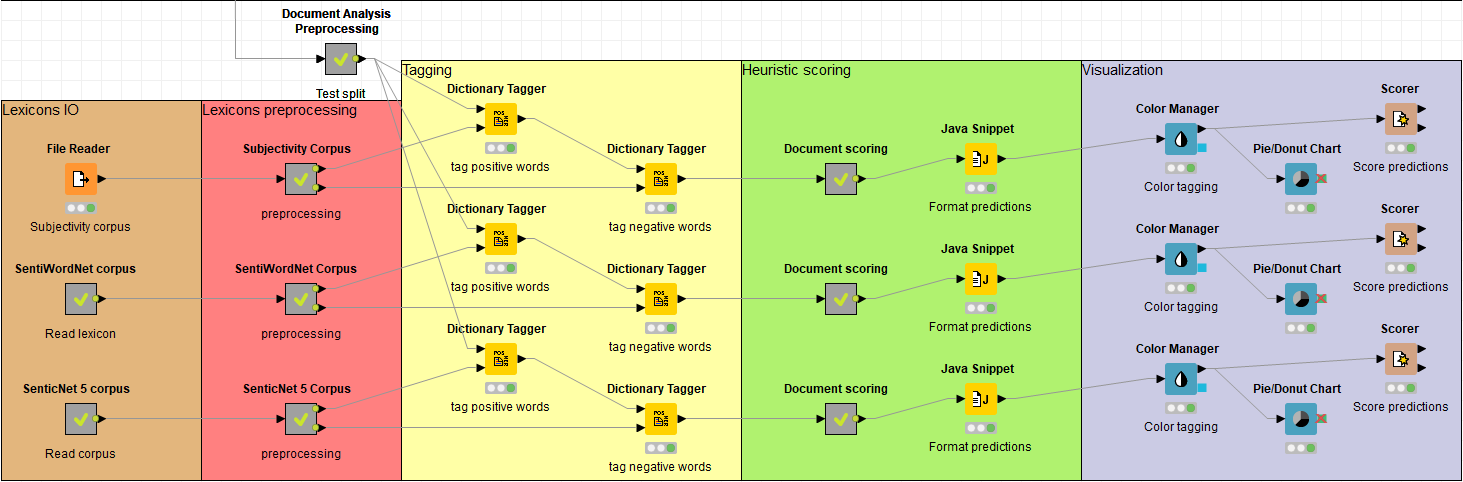
\includegraphics[width=.95\linewidth]{img/analysis/workflow.png}
    \caption{Workflow general del análisis de sentimientos.}
\end{figure}

Para hacer una comparación justa de resultados, se aplica el análisis de sentimientos a la misma partición de test con la que se evalúan los métodos de clasificación.

Como preprocesamiento de los documentos aplicamos un Part Of Speech tagging y Stanford Lemmatizer para quitar las inflexiones de las palabras.

\subsubsection{Lectura de lexicons}

Para el corpus MPQA se usa el mismo procedimiento proporcionado en clase.
Para SentiWordNet, puesto que cada fila puede contener más de un sinónimos, se separan cada uno en una nueva fila con los mismos valores de sentimiento.

Como preprocesamiento, SenticNet únicamente se separa en base a la etiqueta proporcionada.

Para SentiWordNet calculamos el valor de objetividad como $1 - (POS + NEG)$ y a cada término le asignamos un valor \textbf{neutral} si ambos \textit{PosScore} y \textit{NegScore} son iguales, en otro caso le asignamos la etiqueta con el score más alto.

\begin{figure}[t]
    \center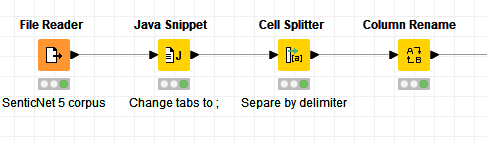
\includegraphics[width=.95\linewidth]{img/analysis/senticnet-reading.png}
    \caption{Lectura del lexicon SenticNet.}
\end{figure}

\begin{figure}[t]
    \center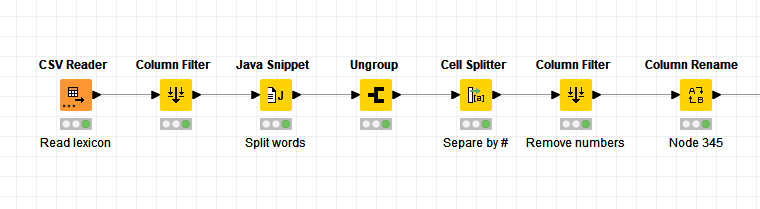
\includegraphics[width=.95\linewidth]{img/analysis/sentiword-reading.png}
    \caption{Lectura del lexicon SentiWordNet.}
\end{figure}

Posteriormente asignamos a cada documento el sentimiento en base al mayor número de palabras que tenga de uno u otro.

% -----------

\subsection{Resultados}

\begin{figure}[t]
    \center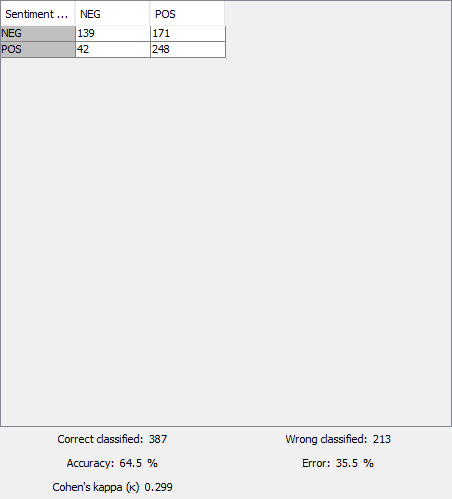
\includegraphics[width=.95\linewidth]{img/analysis/score1.png}
    \caption{Matriz de confusión con MPQA.}
\end{figure}

\begin{figure}[t]
    \center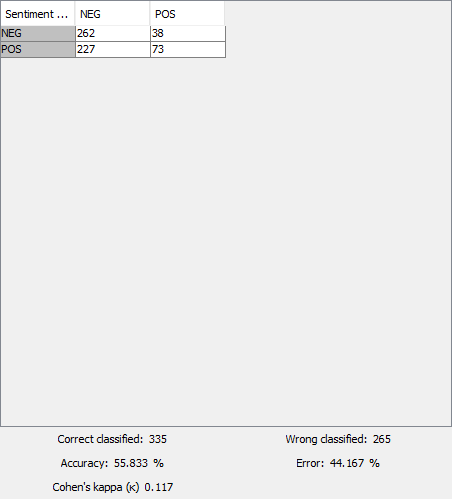
\includegraphics[width=.95\linewidth]{img/analysis/score2.png}
    \caption{Matriz de confusión con SentiWordNet.}
\end{figure}

\begin{figure}[t]
    \center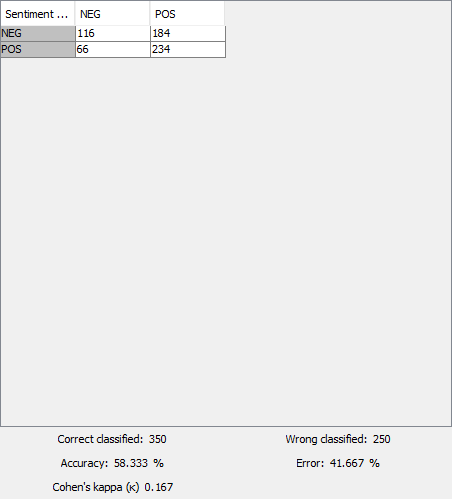
\includegraphics[width=.95\linewidth]{img/analysis/score3.png}
    \caption{Matriz de confusión con SenticNet.}
\end{figure}


\begin{figure}[t]
    \center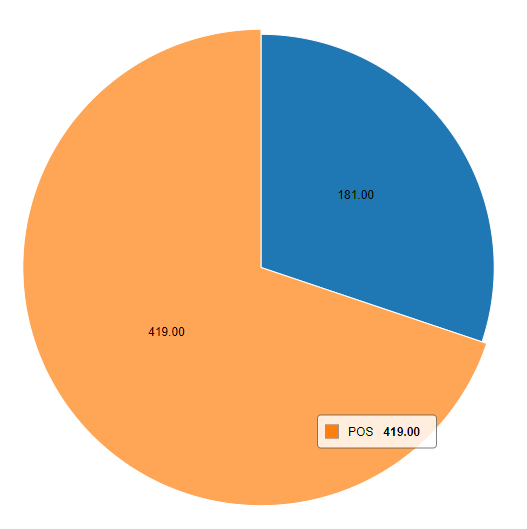
\includegraphics[width=.95\linewidth]{img/analysis/pie1.png}
    \caption{Pie chart con MPQA.}
\end{figure}

\begin{figure}[t]
    \center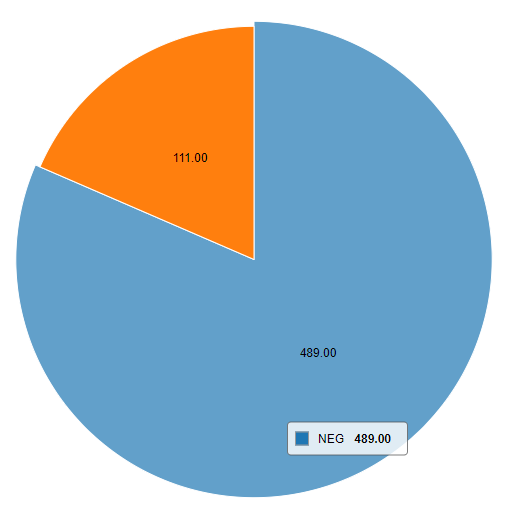
\includegraphics[width=.95\linewidth]{img/analysis/pie2.png}
    \caption{Pie chart con SentiWordNet.}
\end{figure}

\begin{figure}[t]
    \center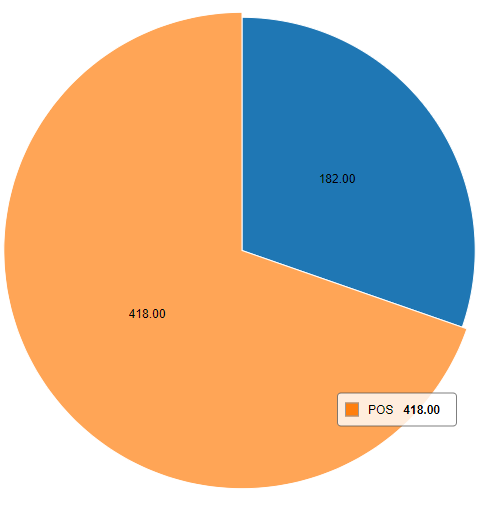
\includegraphics[width=.95\linewidth]{img/analysis/pie3.png}
    \caption{Pie chart con SenticNet.}
\end{figure}